\chapter{Evaluation}
\label{Evaluation}
% GEÄNDERT: Vorlagentext entfernt; Evaluationsdesign vor der Umsetzung festgelegt (Betreueranmerkungen S4/S5)

% NEU: Kapiteleinleitung
Dieses Kapitel legt dar, wie der in Kapitel~\ref{Implementierung} beschriebene Prototyp evaluiert wird, um zu bestimmen, in welchem Grad die Forschungsfrage beantwortet wird. Da die Forschungsfrage mit \glqq inwieweit\grqq{} formuliert ist, zielt die Evaluation nicht auf ein einzelnes Gesamturteil, sondern auf den Grad der Beantwortung jeder der vier Teilfragen aus Abschnitt~\ref{sec:problem-ff}. Das Evaluationsdesign wurde vor der Durchführung festgelegt, damit die Kriterien nicht nachträglich an die Ergebnisse angepasst werden können.

\section{Evaluationsdesign}
\label{sec:eval-design}

\subsection{Evaluationsziele und Bezug zur Forschungsfrage}
\label{subsec:eval-ziele}

% NEU (Betreueranmerkung S5: wie und inwiefern Evaluationsziele und Metriken die FF beantworten)
Jede Teilfrage wird in ein Evaluationsziel überführt, dem eine Kennzahl, ein Erhebungsinstrument sowie eine dreistufige Bewertung zugeordnet sind. Eine Teilfrage gilt als beantwortet, als teilweise beantwortet oder als nicht beantwortet, je nachdem, welche Ausprägung die Kennzahl über die Testfälle hinweg erreicht. Tabelle~\ref{tab:eval-ziele} fasst diese Zuordnung zusammen, und Abbildung~\ref{fig:evaluation} stellt dar, wie aus den Ergebnissen der Grad der Beantwortung abgeleitet wird.

\begin{table}[htbp]
\centering
\caption{Zuordnung der Teilfragen zu Evaluationszielen, Kennzahlen und Bewertungsstufen}
\label{tab:eval-ziele}
\small
\begin{tabular}{p{1.9cm}p{3.0cm}p{3.0cm}p{4.3cm}}
\toprule
\textbf{Teilfrage} & \textbf{Evaluationsziel} & \textbf{Kennzahl} & \textbf{Bewertung (beantwortet / teilweise / nicht)} \\
\midrule
TF1 Erschließen & Die einschlägigen Tabellen werden gefunden & Trefferquote (Recall@k) der Soll-Tabellen; Genauigkeit (Precision@k) & alle Soll-Tabellen in allen Testfällen / in der Mehrzahl der Testfälle / in weniger als der Hälfte \\
TF2 Interpretieren & Die fachliche Deutung ist korrekt & Anteil korrekter Aussagen gegenüber der Referenzantwort & ohne falsche Aussage / falsche Aussagen nur als Interpretation gekennzeichnet / ungekennzeichnete falsche Aussagen \\
TF3 Belegen & Jede Aussage ist rückführbar; Enthaltung bei dünner Evidenz & Anteil auflösbarer Belege; Wert-Exaktheit; Anteil berechtigter Enthaltungen & jede Aussage belegt und jede nötige Enthaltung erfolgt / einzelne Lücken / systematische Lücken \\
TF4 Abweichung & Abweichungen werden korrekt ausgewiesen & Anteil korrekt ausgewiesener Abweichungen gegenüber der Referenz & vollständig und korrekt / unvollständig, aber ohne falsche Abweichung / falsche Abweichungen \\
\bottomrule
\end{tabular}
\end{table}
% [FESTZULEGEN vor Durchführung] Die Stufengrenzen sind ein Vorschlag und vor der ersten summativen Messung verbindlich zu bestätigen (Wert von k, Zahl der Testfälle).

% NEU
Die vier Teilfragen werden bewusst nicht zu einer Gesamtkennzahl verdichtet. Dies liegt darin begründet, dass die Teilfragen den in Abschnitt~\ref{sec:loesung} unterschiedenen Ebenen Retrieval, Zugriff sowie Grounding zugeordnet sind, die jeweils eigene Fehlerarten aufweisen, sodass eine Verdichtung die Zuordnung einer Abweichung zu ihrer Entstehungsebene aufheben würde. Der Grad der Beantwortung der Forschungsfrage ergibt sich stattdessen aus dem Profil der vier Teilfragen: Die Forschungsfrage gilt als weitgehend beantwortet, wenn sämtliche Teilfragen mindestens teilweise beantwortet sind und TF3 vollständig beantwortet ist, da die Belegbarkeit den Kern des Beitrags bildet. Die Diskussion in Abschnitt~\ref{sec:eval-diskussion} ordnet das Profil anschließend ein.

\begin{figure}[htbp]
	\centering
	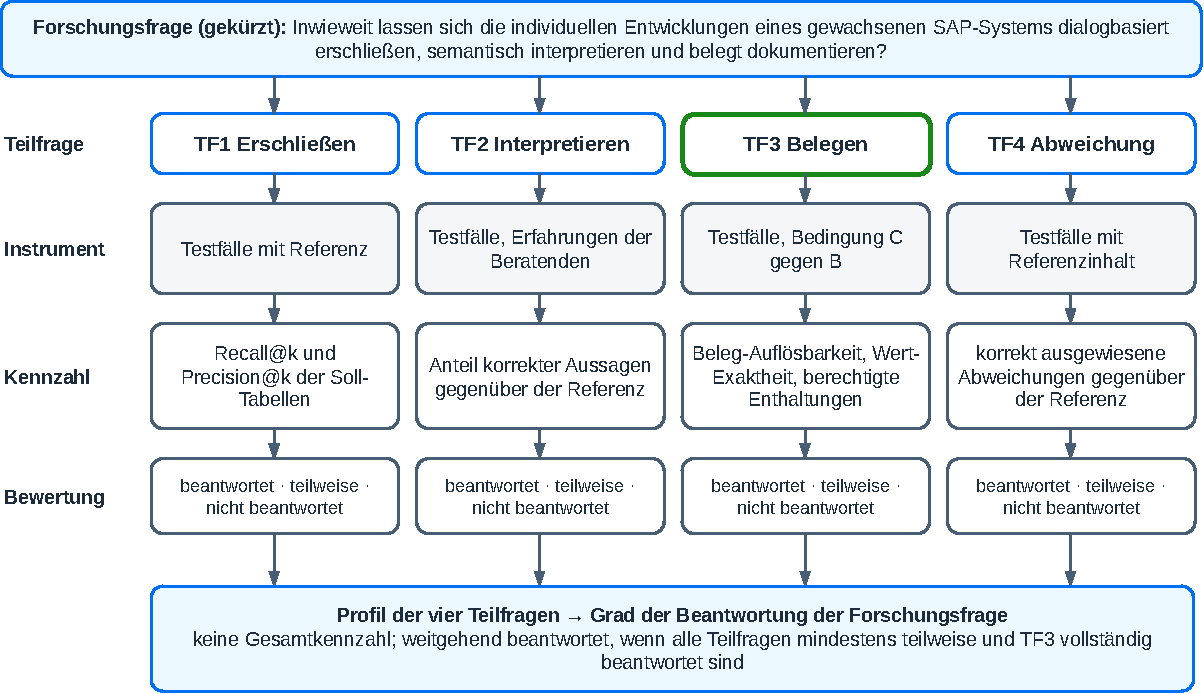
\includegraphics[width=\linewidth]{Grafiken/abb5_1_evaluation.pdf}
	\caption{Ableitung des Grads der Beantwortung der Forschungsfrage aus den Teilfragen, Kennzahlen und Erhebungsinstrumenten (eigene Darstellung).}
	\label{fig:evaluation}
\end{figure}

% NEU: Einordnung nach FEDS
Die Evaluation kombiniert zwei Zugänge, die sich nach der Unterscheidung von Venable et al. als künstliche sowie naturalistische Evaluation einordnen lassen \cite{venable_feds_2016}. Die künstliche Evaluation erfolgt an vorab festgelegten Testfällen mit bekannter Referenzantwort und liefert die Kennzahlen der Tabelle~\ref{tab:eval-ziele}. Die naturalistische Evaluation erfolgt über die Erfahrungen von Beratenden mit dem Werkzeug im Arbeitsalltag und prüft, ob sich die an den Testfällen gemessene Qualität unter realen Fragen bestätigt. Beide Zugänge begleiten die Entwicklung zunächst formativ, indem gefundene Fehler einer Fehlerklasse zugeordnet und behoben werden, und münden in eine abschließende summative Messung.

\subsection{Bedingungen}
\label{subsec:eval-bedingungen}

% NEU (übernommen aus Textbaustein 10.09.2026)
Ein Vergleich mit und ohne Grounding, wie ihn das Exposé vorsieht, vermengt zwei Wirkmechanismen: den bloßen Zugriff auf Systemdaten und den Grounding-Mechanismus im Sinne der Belegpflicht sowie der Prüfung. Um beide zu trennen, wird die Versuchsanordnung auf vier Bedingungen erweitert, die in Tabelle~\ref{tab:bedingungen} dargestellt sind.

\begin{table}[htbp]
\centering
\caption{Bedingungen der Versuchsanordnung}
\label{tab:bedingungen}
\footnotesize
\begin{tabular}{p{1.8cm}p{2.3cm}p{1.9cm}p{1.4cm}p{3.9cm}}
\toprule
\textbf{Bedingung} & \textbf{Datenzugriff} & \textbf{Belegpflicht} & \textbf{Prüfung} & \textbf{Isolierter Effekt} \\
\midrule
A & nein & -- & -- & Wissen des Modells ohne Systemzugriff \\
B & ja & nein & nein & Effekt des reinen Datenzugriffs \\
C & ja & ja & ja & Effekt des Groundings als Differenz zu B \\
D & Soll-Belege vorgegeben & ja & -- & Obergrenze bei fehlerfreier Erschließung \\
\bottomrule
\end{tabular}
\end{table}

% NEU
Die Differenz zwischen den Bedingungen C und B weist den Beitrag des Groundings aus und beantwortet damit den Kern der Teilfrage~TF3, während die Differenz zwischen B und A den Beitrag des Systemzugriffs abbildet. Bedingung~D trennt Fehler der Erschließung von Fehlern der Interpretation, da hier die Soll-Tabellen vorgegeben werden. Bedingung~A dient dabei nicht als ernsthafte Alternative, da ein Sprachmodell ohne Systemzugriff über ein unbekanntes Kundensystem keine prüfbare Aussage treffen kann, sondern als Nachweis, welcher Anteil einer Antwort allein aus allgemeinem Wissen über den SAP-Standard stammt.

\subsection{Testfälle}
\label{subsec:eval-testfaelle}

% NEU (Grundlage: Testfalldokumentation und tests/cases.py)
Als Testfälle dienen drei Fälle steigender Schwierigkeit, die jeweils eine andere Anforderung an den Ansatz stellen. Der erste Fall betrifft reines Customizing und wird in drei Stufen abgefragt, von der Frage nach den vorhandenen Regelgruppen über die Antragsarten je Regelgruppe bis zu der Frage, welche Antragsarten Auszubildenden zur Verfügung stehen, die das durchgängige Beispiel dieser Arbeit bildet. Der zweite Fall erfordert zusätzlich die Auflösung einer Erweiterungsimplementierung, die nur für einen bestimmten Untertyp wirksam ist. Der dritte Fall verbindet eine Erweiterung mit Standard- und kundendefinierten Tabellen sowie einer erst zur Laufzeit aufgelösten Merkmalsauswertung und dient der Darstellung der Grenzen des Ansatzes.

% NEU
Zu jedem Testfall wird vor der Messung eine Referenzantwort erstellt, die aus den erwarteten Tabellen, den erwarteten Aussagen sowie den erwarteten Abweichungen besteht. Jede Aussage der Referenzantwort wird dabei selbst am System geprüft, indem die zugehörige Tabellenzeile gelesen wird, sodass die Referenz nicht auf einer Einschätzung, sondern auf dem Systemzustand beruht. Da Sprachmodelle bei identischer Eingabe unterschiedliche Ausgaben erzeugen können, wird jeder Testfall je Bedingung mehrfach ausgeführt. % [FESTZULEGEN: Anzahl der Wiederholungen]

\subsection{Kennzahlen je Ebene und Fehlertaxonomie}
\label{subsec:eval-metriken}

% NEU (Textbausteine 10.09. und 11.09.2026)
Die Kennzahlen werden je Ebene erhoben. Auf der Ebene des Retrievals werden Trefferquote sowie Genauigkeit der gefundenen Tabellen gegenüber den Soll-Tabellen gemessen, wobei nicht gefundene Tabellen gesondert erfasst werden, da die Eingrenzung des Korpus diese Fehlerart begünstigt. Auf der Ebene des Zugriffs wird die Erfolgsquote der Werkzeugaufrufe erhoben. Auf der Ebene des Groundings werden die Auflösbarkeit der Belege, die Übereinstimmung der genannten Werte mit den gelesenen Werten sowie der Anteil berechtigter und unberechtigter Enthaltungen gemessen. Diese Kennzahlen werden deterministisch ermittelt. Auf eine Bewertung durch ein Sprachmodell wird verzichtet, um eine zirkuläre Prüfung auszuschließen.

% NEU
Ergänzend wird jeder gefundene Fehler einer vorab festgelegten Fehlerklasse zugeordnet, sodass sich Einzelbeobachtungen zu einer Aussage über die Schwachstellen des Ansatzes verdichten lassen. Tabelle~\ref{tab:fehlerklassen} stellt die Klassen dar.

\begin{table}[htbp]
\centering
\caption{Fehlertaxonomie der Evaluation}
\label{tab:fehlerklassen}
\small
\begin{tabular}{p{1.3cm}p{4.0cm}p{7.0cm}}
\toprule
\textbf{Klasse} & \textbf{Bezeichnung} & \textbf{Beschreibung} \\
\midrule
F1 & falsch-positives Retrieval & eine fachfremde Tabelle wird als relevant eingestuft \\
F2 & falsch-negatives Retrieval & eine einschlägige Tabelle wird nicht gefunden \\
F3 & erfundener Bezeichner & eine genannte Tabelle oder ein Feld existiert nicht \\
F4 & Wertwiderspruch & eine Aussage widerspricht dem gelesenen Wert \\
F5 & unbelegte Interpretation & eine plausible Aussage ohne Deckung in den abgerufenen Daten \\
F6 & fehlende Enthaltung & das System antwortet, obwohl die Evidenz nicht ausreicht \\
F7 & Kontext- und Größenfehler & ein Objekt überschreitet das Kontextfenster \\
F8 & fehlerhafte Schlüsselauflösung & ein existierender Schlüssel wird einem existierenden, jedoch nicht zugehörigen Klartext zugeordnet \\
\bottomrule
\end{tabular}
\end{table}

\subsection{Erfahrungen der Beratenden mit dem Werkzeug}
\label{subsec:eval-erfahrungen}

% NEU (Entscheidung R4: ersetzt die im Exposé vorgesehenen Experteninterviews bzw. die Beraterbewertung)
Die naturalistische Evaluation erfolgt über die Erfahrungen von Beratenden des Kooperationspartners, die den Prototyp für eigene Fragen an ein ihnen unbekanntes Customizing einsetzen. Jede Nutzung wird in einem strukturierten Protokoll festgehalten, das die gestellte Frage, die erhaltene Antwort, das Ergebnis der eigenen Nachprüfung der Belege, die Einschätzung der Antwort als korrekt, teilweise korrekt oder falsch sowie den geschätzten Zeitaufwand einer manuellen Klärung umfasst. Abschließend beschreiben die Beratenden in einer kurzen Befragung, in welchen Situationen das Werkzeug ihre Arbeit unterstützt hat und in welchen nicht. % [FESTZULEGEN: Zahl der Beratenden, Zeitraum, Protokollvorlage im Anhang]

% NEU
Dieser Zugang ergänzt die Testfälle in zweierlei Hinsicht. Er prüft die Teilfrage~TF2 an Fragen, die nicht vom Verfasser der Arbeit formuliert wurden, und er zeigt, ob die dialogbasierte Erschließung den Aufwand der manuellen Exploration tatsächlich verringert, wie es die Problemstellung voraussetzt. Gegenüber Experteninterviews liegt sein Vorteil darin, dass die Bewertung an einer konkreten Antwort des Werkzeugs erfolgt und nicht an einer allgemeinen Einschätzung des Ansatzes.

\subsection{Limitationen der Evaluation}
\label{subsec:eval-limitationen}

% NEU (Betreueranmerkung S5: Limitationen der Evaluation bereits hier anführen)
Die Aussagekraft der Evaluation ist durch mehrere Faktoren begrenzt, die bereits vor der Durchführung feststehen:
\begin{itemize}
	\item \textbf{Einzelsystem:} Sämtliche Messungen erfolgen an einem einzelnen SAP-System, sodass die Ergebnisse nicht ohne weitere Erhebung auf andere Systemlandschaften übertragbar sind.
	\item \textbf{Zahl der Testfälle:} Die geringe Zahl der Testfälle erlaubt Aussagen über das Verhalten in diesen Fällen, jedoch keine statistisch gesicherte Verallgemeinerung.
	\item \textbf{Referenzantworten:} Die Referenzantworten werden vom Verfasser erstellt. Dem wird dadurch begegnet, dass jede Referenzaussage am System geprüft wird, die Auswahl der erwarteten Aussagen bleibt jedoch eine Einschätzung.
	\item \textbf{Beratende des Kooperationspartners:} Die Beratenden stammen aus dem Unternehmen, in dessen Kooperation die Arbeit entsteht, sodass ihre Einschätzung nicht unabhängig ist.
	\item \textbf{Nichtdeterminismus:} Die Ausgaben des Sprachmodells schwanken zwischen Läufen, was durch Wiederholungen nur abgeschwächt wird.
	\item \textbf{Referenzinhalt des Standards:} Die Bewertung der Teilfrage~TF4 setzt voraus, dass der ausgelieferte Referenzinhalt am Zielsystem lesbar ist.
\end{itemize}

\section{Durchführung}
\label{sec:eval-durchfuehrung}
% TODO: Ablauf, Zeitraum, eingesetzte Modellversion, Zahl der Läufe, Protokollierung

\section{Ergebnisse}
\label{sec:eval-ergebnisse}
% TODO: Ergebnisse je Teilfrage, je Bedingung und je Testfall; Fehlerprotokoll nach F1-F8; Auswertung der Werkzeugerfahrungen

\section{Interpretation und Diskussion}
\label{sec:eval-diskussion}
% TODO: Profil der Teilfragen einordnen; Entwurfsentscheidungen kritisch reflektieren (Leitfaden: wichtige Entscheidungen am Ende hinterfragen)
